\chapter{The CMS Detector\label{ch:CMS}}

CMS is one of the largest scientific collaborations in the history of mankind with over 4,000 participants from 42 countries and 182 institutions.
The CMS experiment is one of four detectors built at crossing sites of the LHC beams, and is one of two general purpose detectors (the other being the ATLAS detector) which have been designed to exploit the physics opportunities presented by the LHC.
It is designed to investigate various physical phenomena concerning the SM and beyond it, such as Supersymmetry, Extra Dimensions and Dark Matter.

The CMS detector essentially acts as a giant super highspeed camera that makes 3D images of the collisions that are produced at a rate of 40~\unit{MHz}.
As its name implies, the detector is a solenoid that is constructed around a superconducting magnet capable of producing a magnetic field of 3.8~\unit{\tesla}.
The magnetic coil is 13~\unit{m} long with an inner diameter of 6~\unit{m}, making it the largest superconducting magnet ever constructed.
The CMS detector itself  (as shown in \autoref{CMSLayout}) is over 28~\unit{m} long with a diameter of 15~\unit{m} and it has a weight of approximately 14,000~\unit{\tonne}.
Within the solenoid volume are a silicon pixel and strip tracker, a lead tungstate crystal electromagnetic calorimeter (ECAL), and a brass and scintillator hadron calorimeter (HCAL), each composed of a barrel and two endcap sections. Forward calorimeters extend the coverage of a coordinate known as the pseudorapidity ($\eta$) (see \Cref{fig:CMSCoord}) provided by the barrel and endcap detectors. Muons are measured in gas-ionization detectors embedded in the steel flux-return yoke outside the solenoid.

\begin{figure}
	\centering
	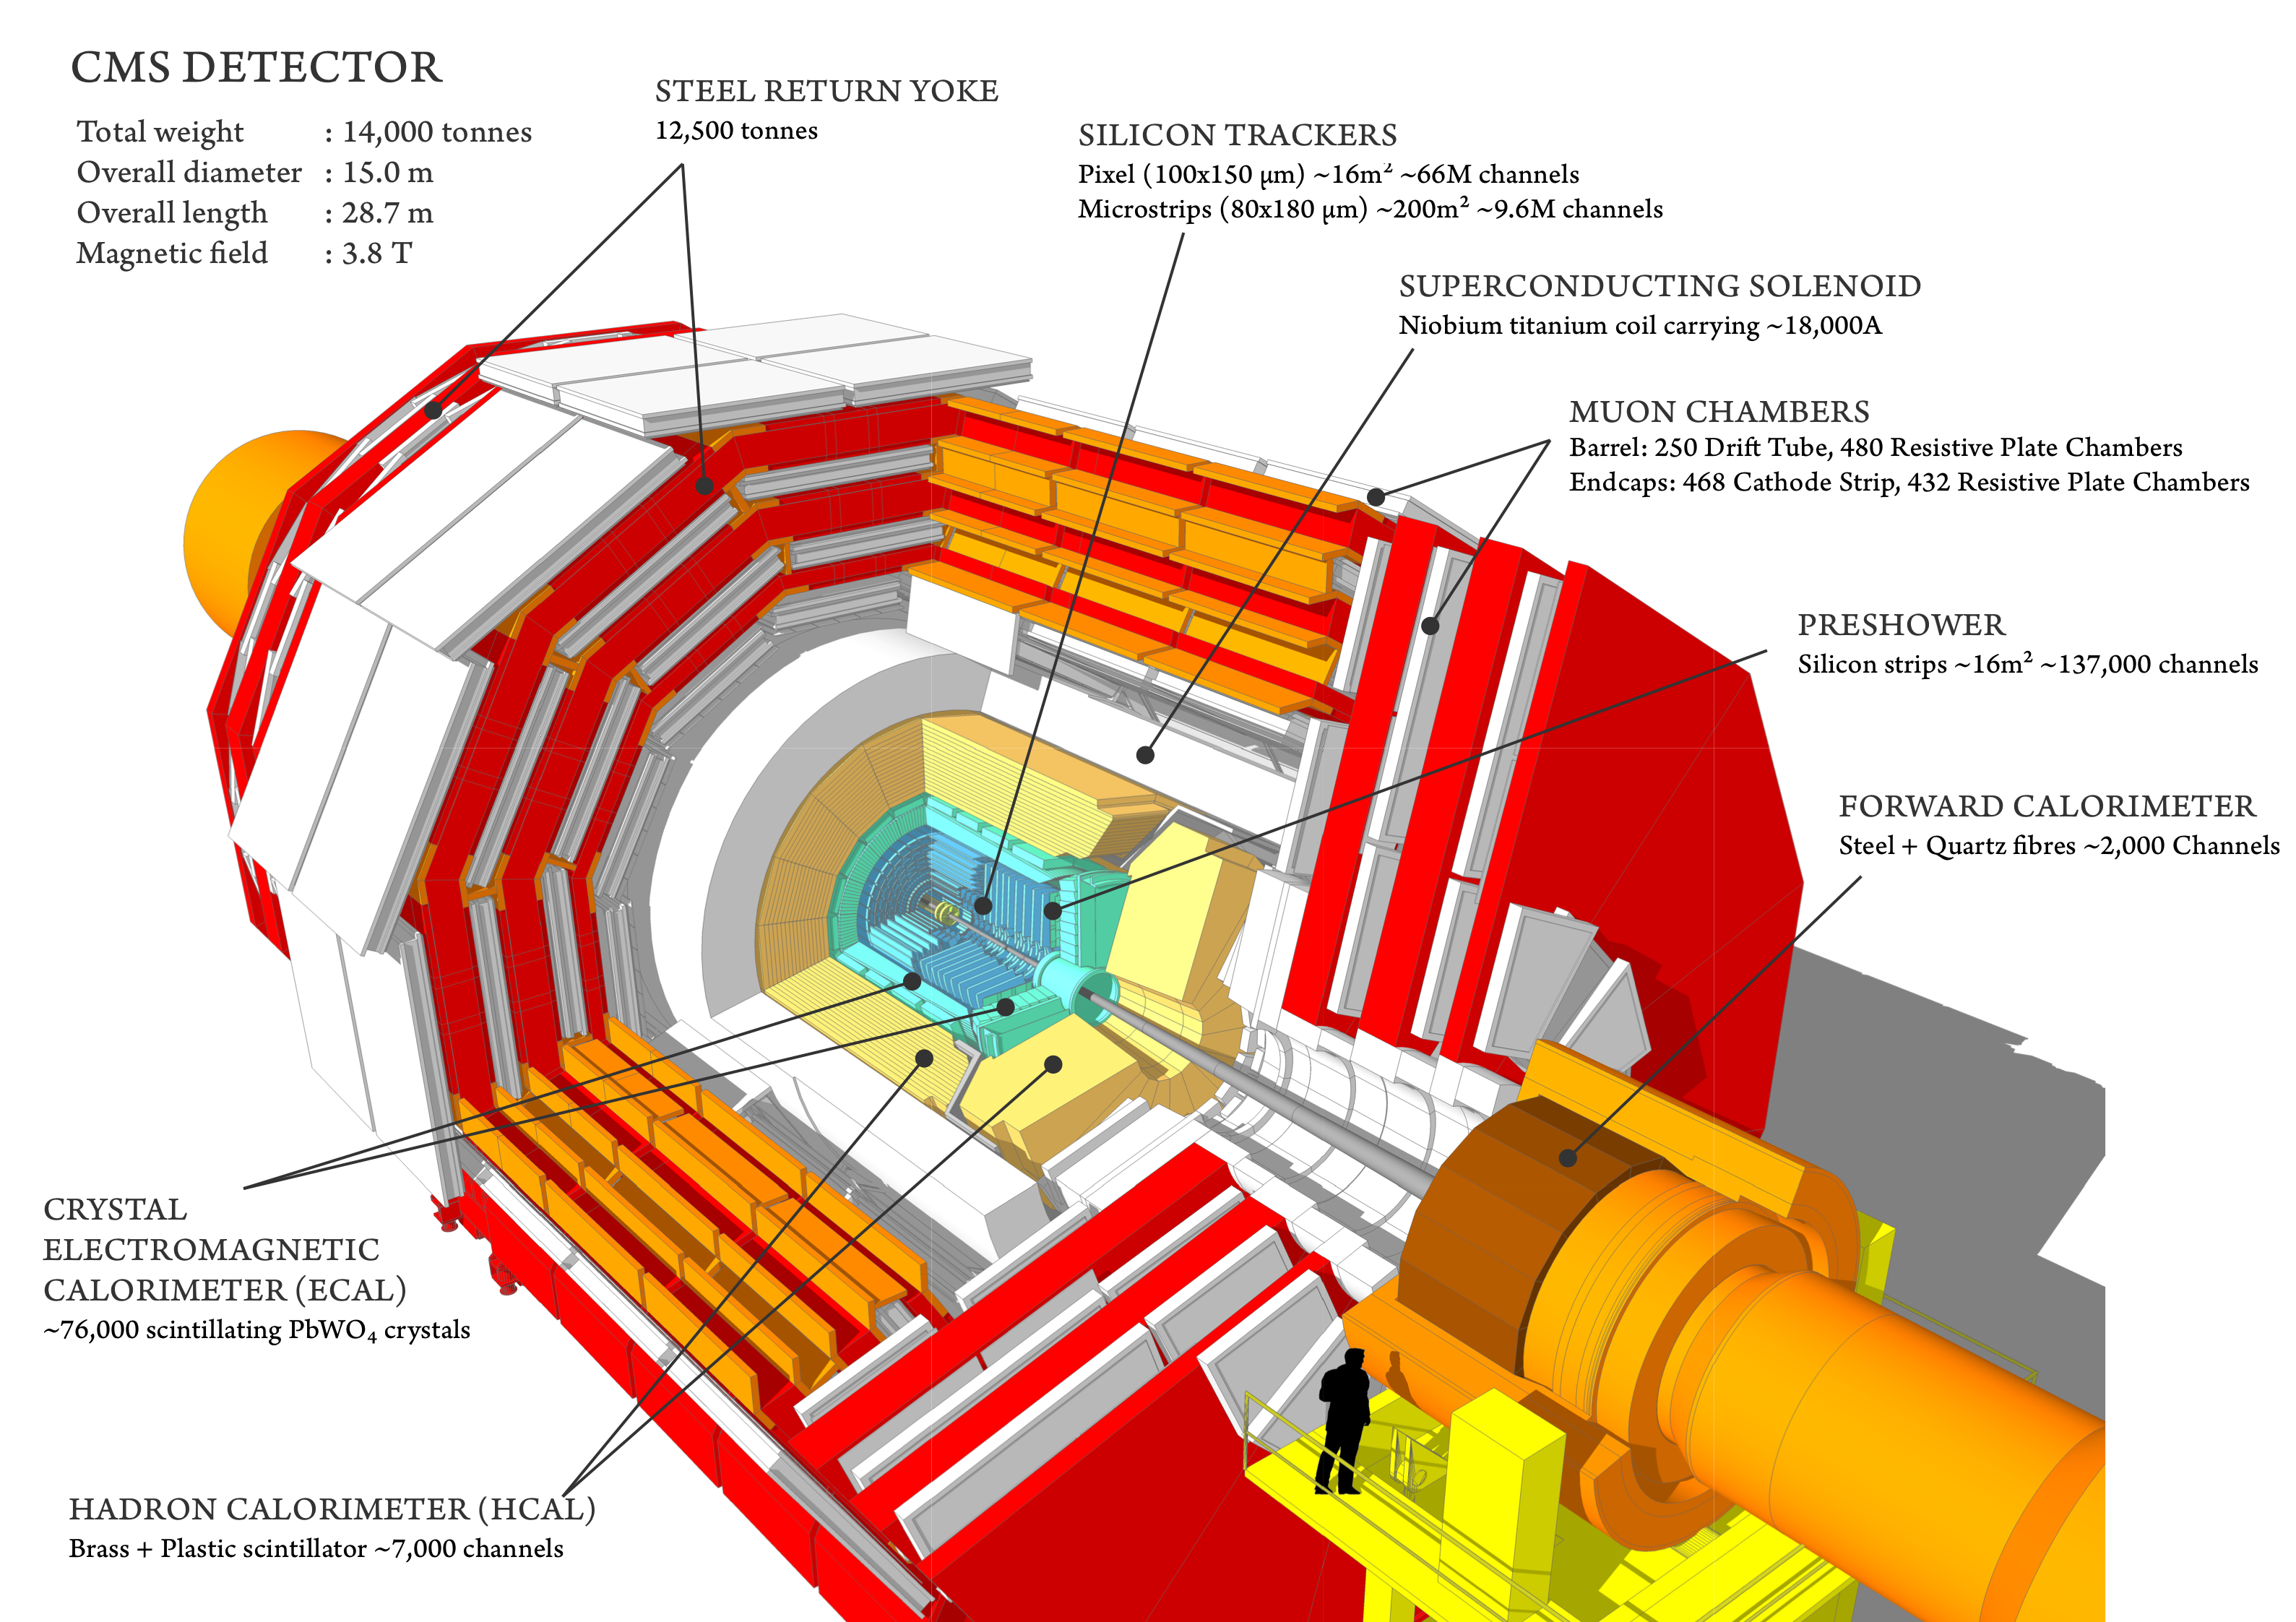
\includegraphics[width=\linewidth]{CMSLayout.png}
	\caption[CMS Detector]{The CMS Detector \cite{CMS_detector}}
	\label{CMSLayout}
\end{figure}
\begin{figure}
	\centering
	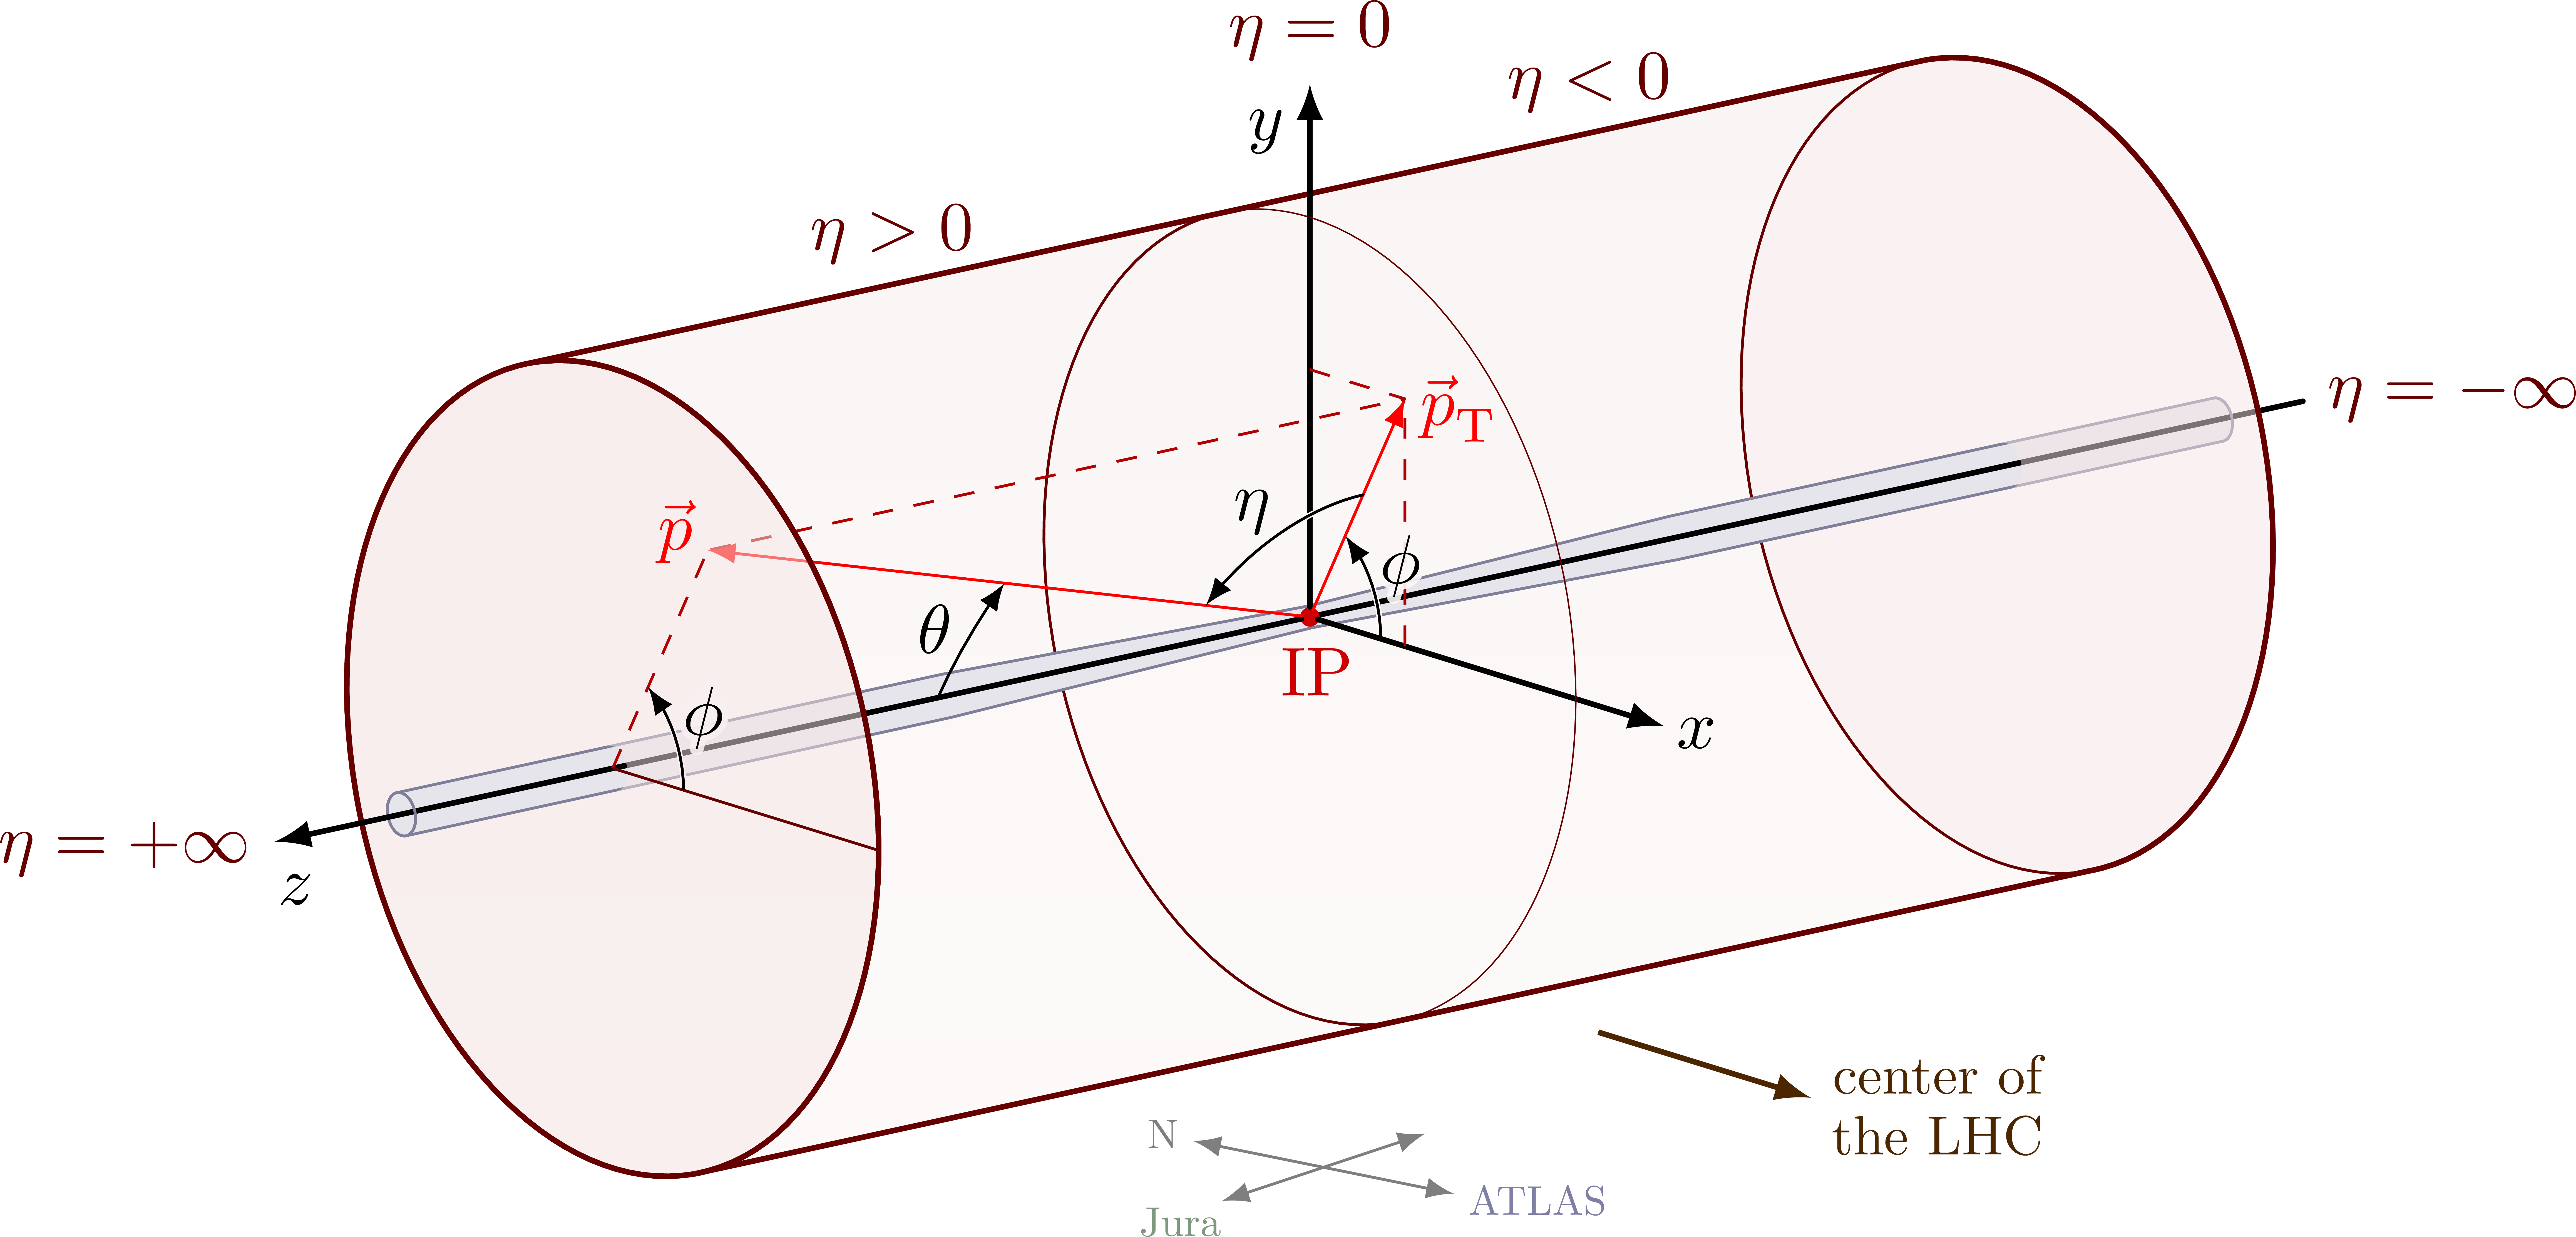
\includegraphics[width=.8\linewidth]{Images/CMS Coordinate.png}
	\caption[The CMS coordinate system]{The CMS coordinate system. From \cite{CMS_detector}}
	\label{fig:CMSCoord}
\end{figure}
The detector has an onion-like structure to capture all the particles that are produced in high-energy collisions.
A property of these particles that is exploited is their charge. Normally, particles produced in collisions travel in a straight line, but in the presence of a magnetic field, their paths are curved.
Except for the muon system, the rest of the sub-detectors lie inside the 3.8~\unit{T} magnetic field.
The Tracking devices are responsible for drawing the trajectory of the particles by using a computer program that reconstructs the path using electrical signals that are left by the particles as they move. The Calorimeters measure the energy of particles that pass through them by absorbing their energy with the intent of stopping them.
The particle identification detectors work by detecting radiation emitted by charged particles and using this information they can measure the speed, momentum, and mass of a particle. After the information is put together to make the “snapshot” of the collision one looks for results that do not fit the current theories or models in order to look for new physics.

\autoref{CMSLayers} depicts the particle detection process in CMS. Charged particles leave signatures in the inner tracking system, and the vertices from decaying short-lived particles can be identified. Photons, electrons, neutral pions and kaons are stopped in the crystals of the electromagnetic calorimeter (ECAL) and the scintillation light is used to determine the deposited energy. Hadrons punch through further and are generally stopped by the hadronic calorimeter (HCAL), where jets are confined and only the highest-energy hadrons and muons pass through the superconducting solenoid into the outer regions of the CMS barrel. Finally, muons are detected in the various muon detectors which interleave the return yoke of the magnet. Neutrinos escape from the CMS detector and are inferred from an imbalance of energy in the reconstructed event called missing transverse energy (MET or $\vec{p}_T^{\text{miss}}$).
More detailed descriptions of the CMS detector, together with a definition of the coordinate system used and the relevant kinematic variables, can be found in~\cite{CMS:2008xjf,CMS:2023gfb}.

\begin{figure}[h]
	\centering
	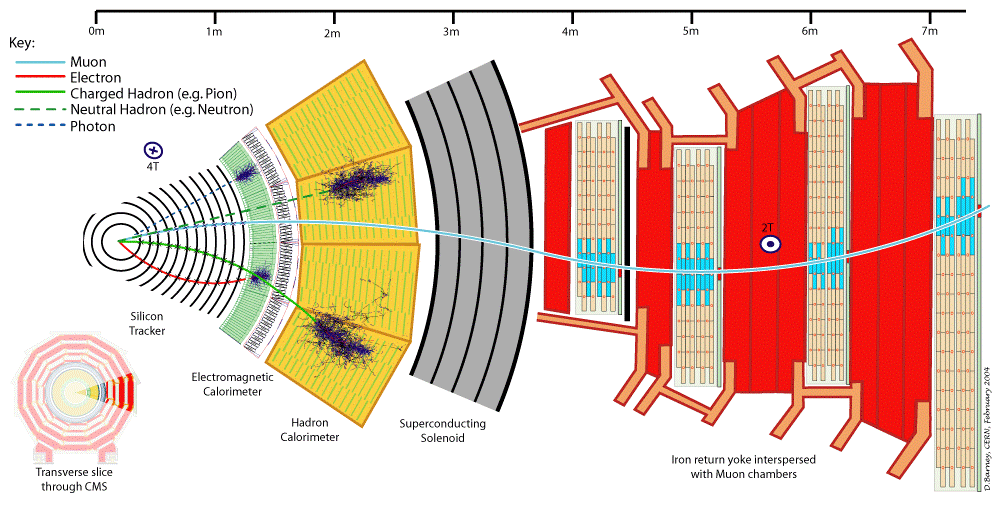
\includegraphics[width=.9\linewidth]{CMSLayers.png}
	\caption[Particle trajectories and footprint in CMS]{The trajectory of a particle traveling through the layers of the detector leaving behind it's signature footprint\label{CMSLayers}}
\end{figure}



% The project focusses specifically on data collected from one of the Calorimeters, - the Hadron Calorimeter (HCAL). The HCAL, as its name indicates, is designed to detect and measure the energy of hadrons or, particles that are composed of quarks and gluons, like protons and neutrons. Additionally, it provides an indirect measurement of the presence of non-interacting, uncharged particles such as neutrinos (missing energy) . Measuring these particles is important as they can tell us if new particles such as the Higgs boson or supersymmetric particles (much heavier versions of the standard particles we know) have been formed. The layers of the HCAL are structured in a staggered fashion to prevent any gaps that a particle might pass through undetected. There are two main parts: the barrel and the end caps. There are 36 barrel wedges that form the last layer of the detector inside the magnet coil, there is another layer outside this, and on the endcaps, there are another 36 wedges to detect particles that come out at shallow angles with respect to the beam line.
